% Do NOT change this "Section" title
% and do NOT add more "Section" level titles.
\section{Implementation}\label{sec:implementation}
Overview of the motor and motor controller system:
\begin{figure}[h]
    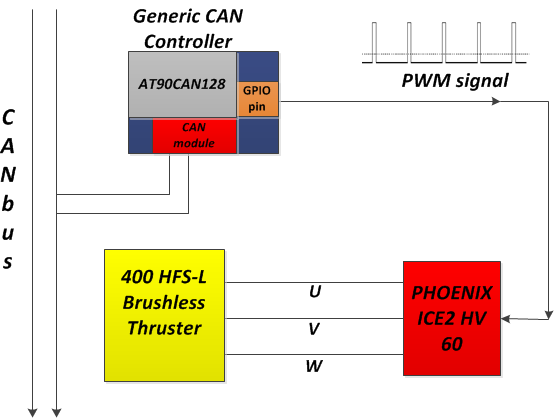
\includegraphics[width=0.5\textwidth]{./figure/figA.png}
    \caption{Motor and motor controller system overview}
    \label{fig:one_column_figure}
\end{figure}

The implementation has the following parts:
\begin{itemize}
\item Thrusters
\item Thruster speed controller
 \item CAN message processing
 \item Generating the PWM signal
 \item Main program 
\end{itemize}

% You can use how many "subsections" and "subsubsections" you like.
\subsection{Thrusters}
During the selection of thrusters only two models seemed to satisfy the needs of Naiad. One was the SeaBotix BTD150 which is a very popular brushed DC thruster. The other one was the CrustCrawler 400HFSL brushless DC thruster which is not as popular as the first one and a little more expensive. After the advantages and disadvantages were considered the CrustCrawler 400HFS-L has been decided to be the better option for Naiad by being lighter, more power efficient and more powerfull than the SeaBotix BTD150. 

\begin{table}[h]
\centering
    \caption{CrustCrwler 400 HFS-L specifications}
    \begin{tabular}{|c|c|} \hline
    \label{table:one_column}
       Motor type    &  High efficiency brushless \\ \hline
       Weight(motor) & 185 g \\ \hline
         Weight(thruster) & 255 g \\ \hline
           Max power &  130 W \\ \hline
             Gear ratio & 4.28:1 \\ \hline
               Operating voltage & 12 to 50 Volts \\ \hline
                 Depth rating  & 300 ft. \\ \hline
                   Thruster Housing & T-6 Aluminum \\ \hline
                     Thruster length & 15.87 cm \\ \hline  
                      Propeller size & 60 mm \\ \hline
     
    \end{tabular}
\end{table}
 
\subsection{Thrusters speed controller}
The CrustCrawler 400 HFS-L's brushless motor has three windings U, V and W and cannot be connected directly to the Generic CAN controller that has no feature to control brushless motors. So a special speed controller had to be used to actuate the thrusters. After a research and comparison of different brushless controllers a decision was made to go for the one suggested by the thruster manufacturer, and that is the Phoenix ICE2 HV 60 thruster controller. A feature of this brushless controller is that it has a learning function that can calibrate the controller for different systems. 

The speed controllers principle of operation is to take a PWM signal as input
and to convert it in signals for the brushless motor. The input of the
motor controller \cite{web:motor} can be calibrated with the
learning function by holding the throttle in the maximum position
for a few seconds, then  the minimum position, and finally the middle
position. During the power-up the throttle of the speed controller has
to be at the middle position. If during power up  the controller is at
the maximum forward position, the device will  go into the configuration
mode. By moving the throttle to different values the output will change and
will cause the thruster to increase its speed or decrease it depending on
what action has been taken.

\subsection{CAN message processing}
The speed of the thrusters is adjusted several times a second. This is done by receiving messages that contain the actuation value for the thruster from the CAN bus. The received CAN message consists of six bytes out of the maximum of 8 specified in the CAN bus. 

Each of the bytes will represent an actuation value for a thruster. For example the CAN message is received by all the thrusters but each of them will use only one byte from the message. For example the thruster with id one will use the first byte, the thruster with id two will use the value from the second byte and so on. Each byte contains an eight bit signed value but the structure in which the CAN message is saved when it is received is eight bytes of unsigned values. So, for the correct interpretation of the data a conversion has to be made using the Ada Unchecked conversion feature of the Ada programming language. This feature copies the bits from one type of variable and writes them in another type of variable without raising any exceptions if the sizes of the two type are equal or the empty one is bigger.  
\subsection{Generating the PWM signal}
The PWM signal is used to control the speed of the thrusters and also the direction of the thrust (forward or backward). The PWM signal is created by the Generic CAN controller and then fed to the brushless speed controller. The brushless speed controller expects a PWM signal with the pulse width of 1 to 2 ms, every 6 to 25 ms. This PWM signal is created by configuring some registers of the AT90CAN128 MCU.

 The period of the pulse is configured with the ICR1 register and set to 16.3 ms with a resolution of 4096. To generate the pulse another register is used; OCR1A which at each Timer1 increment is compared to the TCNT1 register which keeps track of current number of clock ticks and if they match the value on the output pin is set to 0 and the TCNT1 register is set back to 0. 

\subsection{Main program}
The main program consists of a loop in which the CAN message processing and the generation of the PWM signal is done. Inside the endless loop, the function that reads the CAN messages from the buffer is called, and if there are any available CAN messages in the buffer they will be processed. If not, it will wait for the specified amount of time for a message to be received and then skip to the next instruction.

 
